\documentclass[a4paper,10pt]{article}

\usepackage{amssymb}
\usepackage{amsmath}
\usepackage{amstext}
\usepackage{amsthm}
\usepackage{esint} % more integral signs 
\usepackage{float}
\usepackage{graphicx}
\usepackage[margin=2.0cm]{geometry}
\usepackage{setspace}
\usepackage{url}
\usepackage[skip=2pt]{caption}
\usepackage[nottoc]{tocbibind}

%\setstretch{2.0}

\title{Multi-Domain Finite Element Meshing\\for Parotid Acinar Cell Modeling and Simulation}
\author{John Rugis$^{a,b}$ \and Nathan Pages$^b$ \and David Yule$^c$ \and James Sneyd$^b$}
\date{%
  $^a$corresponding author - email: j.rugis@auckland.ac.nz, phone: 649-923-2313\\%
  $^b$ Department of Mathematics,University of Auckland, Auckland, New Zealand\\%
  $^c$School of Medicine and Dentistry, University of Rochester, Rochester, NY, USA\\[2ex]%
  \today
}

\begin{document}
\maketitle

\section*{Keywords}
multi-domain mesh refinement, surface curvature, volumetric mesh, finite element modeling, parotid acinar cells.\\

\section*{Abstract}
350 words maximum.\\
Contribution: Multi-domain mesh surface smoothing using iterative coupled refinement.\\ 
Refinement termination guided by reference target surface curvature.\\  

\section{Introduction}
The primary role of salivary gland acinar cells is to secrete saliva, the lack of which causes a host of severe medical difficulties \cite{fox1985,melvin1991}. Thus, an understanding of the mechanisms underlying saliva secretion are vital for the understanding of oral health.  The basic mechanism of saliva secretion is well understood \cite{nauntofte1992}, and has been previously modeled in detail \cite{sneyd2003}.\\

However, although much is understood about saliva secretion, important questions, both experimental and theoretical, remain. From the theoretical point of view, one of the most interesting questions is how the structure of the acinar cells affects the properties of the Ca$^{2+}$ waves. Along these lines, we have previously reported our first simulation results obtained using an anatomically accurate three-dimensional parotid acinar cell model \cite{Sneyd2017383}. In that initial investigation, we modeled single non-coupled cells. In this paper, we build on that work, extending our mesh model to multiple (seven), coupled cells.\\   

MORE HERE? Why extend to coupled cells?\\

\section{Design Considerations}
We have been using a straightforward implementation of the Finite Element Method (FEM) \cite{gockenbach2006understanding,Hughes2000,gosz2005finite} for our three-dimentional parotid cell simulations and continue doing so in this latest work. In keeping with relatively common FEM practice, we model the surface of each cell with a triangle mesh, then fill-in the cell interiors with tetrahedrons, which results in a complete volumetric mesh for each cell. In the meshes that we developed for our prior work the cells did not physically contact each other i.e. there was a physical gap between the cells.\\

We have recently extended our mathematical modeling to include dynamic interactions between adjacent cells and this imposed additional demands on our mesh construction. With our new design, each cell now touches one or more other cells, sharing some portion of it's surface. We have chosen to model adjacent cell surfaces with \emph{conformal faces} in which numerous individual triangle mesh faces are shared in common between adjacent cells. Note that this facilitates a fairly straightforward mathematical implementation of the interactions between cells. Because we still need to keep track of what's going on in each cell independently, the overall mesh is thought of as being \emph{multi-domain} (one domain for each cell). \\

As with our prior work, the source data for our acinar cell mesh construction consists of a calibrated confocal microscopy image stack. 
We have 31 images at 1024 by 1024 pixels each with a resolution of approximately 0.069 micro-meters per pixel and a stack spacing of 0.80 micro-meters. \\ 

MORE FROM YULE? CITE YULE?\\

Note that, to maximize transparency and reproducibility, we favor the use of open-source software tools.\\
Our work-flow combines existing tools, building on the work of others whenever possible, along with software tools and utilities that we develop ourselves when existing tools do not suffice.\\

\section{Description of Method}

We've designed an FEM mesh creation work-flow for our purposes that can overall be described as having three sequential steps:
\begin{enumerate}
\item Image segmentation
\item Surface triangulation and refinement
\item Volumetric meshing
\end{enumerate}

\subsection{Image segmentation}

\begin{figure}[H]
\begin{center}
\fbox{\includegraphics[width=0.45\textwidth]{images/cells-stack-16_crop.jpg}}
\hspace{0.5cm}
\fbox{\includegraphics[width=0.45\textwidth]{images/segmented.pdf}}
\end{center}
\caption{Subsection of a microscopy image slice on the left and its segmentation on the right.}
\label{fig:slice}
\end{figure}

By visual inspection, we identified and selected a distinct clump of seven cells within our source data image stack.  This clump spanned thirty of the images and covered a maximum of approximately one-quarter of each image. Segmentation was done manually by tracing the outline of each cell in each image with a distinct color, followed by matched color flood-fill. One-quarter of original image number 16, along with it's segmentation, is shown in Figure \ref{fig:slice}.\\

Note that, with our image stack the ratio of stack spacing to pixel resolution is 11.6 being (0.069/0.80). To bring this closer to a ratio of one-to-one, we reduced the X and Y dimensions in the segmented image stack by a factor of eight using nearest neighbor interpolation (to retain the distinct coloring of each cell) resulting in a pixel spacing of approximately 0.55 micro-meters.  The reduceded images were then combined into a single X-Y-Z TIFF stack for convenience.\\

\subsubsection{Curvature}

We also wanted to extract some information from the segmented image stack about the smoothness of the surface of each cell. We chose line curvature as a shape charateristic indicator. Both line and surface curvature have been used successfully in other work to characterise the surface of objects \cite{Rugis_2005_SCMMD, Rugis_2006_SISCE}. Later in this paper we will describe how we used this characteristic line curvature information as guidance in a cell surface curvature smoothing process.\\

\begin{figure}[H]
\begin{center}
\includegraphics[width=0.55\textwidth]{images/outline.pdf}
\end{center}
\vspace{-5mm}
\caption{A sample segmentation pixel outline in green with smoothed node points in red.}
\label{fig:slice_outline}
\end{figure}

We went back to the 1024 by 1024 segmented images and extracted pixels associated with the closed curve boundary outline for each cell in each  image, then selected the outline containing the maximum number of pixels for each cell as being the closest to a ``great arc" slice through that cell. (This great arc criterion was based on the fact that only the curvature associated with a great arc of of sphere is equal to the sphere mean surface curvature.)\\

Next, considering that fact that image pixels are all located on a regular retangular grid (not very useful for calculating actual local curvature!), a smoothed version of each cell outline was created using a 2D Savitzky-Golay (least-squares) fitting filter \cite{doi:10.1021/ac60214a047}. See Figure \ref{fig:slice_outline} for a sample cell outline showing the original pixel locations as well as the smoothing process result.\\

\begin{figure}[H]
\begin{center}
\includegraphics[width=0.4\textwidth]{images/cell1_curv.pdf}
\includegraphics[width=0.4\textwidth]{images/cell4_curv.pdf}
\end{center}
\caption{Reference curvature histograms for two of the cells.}
\label{fig:ref_histogram}
\end{figure}

Distribution of curvature at every outline point for each of the seven cells.\\

\begin{table}[H]
\begin{center}
\footnotesize
\begin{tabular}{|c|c|}
\hline
cell &curvature std\\
\hline
1 &0.2305\\
2 &0.3567\\
3 & 0.3864\\
4 &0.2832\\
5 &0.6868\\
6 &0.3627\\
7 & 0.4226\\
\hline
\end{tabular}
\end{center}
\caption{The standard deviation of the curvature values (in $\mu \text{m}^{-1}$) for each cell obtained from the microscopy image stack.}
\label{tab:ref_curv}
\end{table}

Standard deviation as a single, although imperfect, metric that characterizes the surface smoothness, and in that sense, shape, of each cell.
Standard deviation is only an unambiguous characterization of a normal distribution.\\ 

\subsection{Surface triangulation and refinement}

\subsubsection{Surface triangulation}

\begin{figure}[H]
\begin{center}
\includegraphics[width=0.8\textwidth]{images/rough.pdf}
\end{center}
\caption{Rough multi-domain surface mesh: all seven cells (left) and three exposed cells (right).}
\label{fig:rough}
\end{figure}

CGAL\\

\subsubsection{Surface smoothing refinement}

\begin{figure}[H]
%no smoothing 
%\includegraphics[width=0.2\textwidth]{images/cell1-C0_crop.png}
\begin{center}
\includegraphics[width=0.9\textwidth]{images/evolution.pdf}
\end{center}
\caption{Cell smoothing evolution, with and without inter-cell coupling.}
\label{fig:cell_morph}
\end{figure}

Smooth the cell surface to minimize surface area while maintaining cell volume.\\
Iterative smoothing process.\\
With and without coupling.\\
Restore volume.\\

\begin{figure}[H]
\begin{center}
\includegraphics[width=0.45\textwidth]{images/cell_surf_100.pdf}
\includegraphics[width=0.45\textwidth]{images/cell_vol_100.pdf}
\end{center}
\caption{Cell surface area and volume evolution over one hundred coupled smoothing interations.}
\label{fig:100_iterations}
\end{figure}

When to stop?\\
When target surface curvature is achieved.\\

\begin{figure}[H]
\begin{center}
\includegraphics[width=0.45\textwidth]{images/cell_curv_std.pdf}
\end{center}
\caption{All of the cells hit the target curvature standard deviation ratio of one after nine iterations.}
\label{fig:curv_std}
\end{figure}

Stop after at least half of the smoothed cells drop below target curvature.\\

\begin{figure}[H]
\begin{center}
\includegraphics[width=0.4\textwidth]{images/cell1_curv_morph.pdf}
\includegraphics[width=0.4\textwidth]{images/cell4_curv_morph.pdf}
\end{center}
\caption{Initial surface curvature distribution in brown and smoothed surface curvature in blue.}
\label{fig:morph_histogram}
\end{figure}

Initial and final surface curvature distribution for two cells.
 
\subsection{Volumetric meshing}

GMSH.\\

\section{Results}

\begin{figure}[H]
\begin{center}
\includegraphics[width=0.8\textwidth]{images/smooth.pdf}
\end{center}
\caption{Fully meshed smoothed cells: three exposed cells (left) and all seven cells (right).}
\label{fig:smooth}
\end{figure}

Simulation results from NATHAN.\\

\section{Discussion}

Challenge of physically accurate mesh model generation given incomplete data.\\
Mesh design constrained by both the practical requirements of finite element modeling and the simplification assumptions made in the mathematical model.\\ 

\section{Conclusion and Future Plans}

Multi-domain conformal mesh for FEM simulation.\\
Confirmed with initial test runs using our calcium dynamics model.\\
Use the meshes in simulations with an updated mathematical model that includes interactions between cells.\\


\section{Acknowledgements}
This work was supported by the National Institutes of Health grant number 5R01DE019245 and by a grant from New Zealand eScience Infrastructure (NeSI).\\

\bibliographystyle{alpha}
\bibliography{references}

\pagebreak
\appendix

\section{Numerical Data}

\begin{table}[H]
\begin{center}
\footnotesize
\begin{tabular}{|c|ccccccccccc|}
\hline
cell & 0 &1 &2 &3 &4 &5 &6 &7 &8 &9 &10\\
\hline
1 &0.1374 &0.0968 &0.0723 &0.0607 &0.0541 &0.0500 &0.0472 &0.0453 &0.0439 &0.0428 &0.0411\\
2 &0.1464 &0.1003 &0.0771 &0.0679 &0.0631 &0.0604 &0.0587 &0.0574 &0.0566 &0.0560 &0.0555\\
3 &0.1315 &0.0901 &0.0694 &0.0591 &0.0531 &0.0493 &0.0467 &0.0447 &0.0432 &0.0420 &0.0411\\
4 &0.1418 &0.0957 &0.0736 &0.0634 &0.0579 &0.0546 &0.0524 &0.0508 &0.0496 &0.0487 &0.0480\\
5 &0.1549 &0.1037 &0.0808 &0.0714 &0.0667 &0.0640 &0.0623 &0.0611 &0.0602 &0.0596 &0.0591\\
6 &0.1407 &0.0939 &0.0713 &0.0610 &0.0552 &0.0516 &0.0492 &0.0475 &0.0461 &0.0451 &0.0443\\
7 &0.1355 &0.0901 &0.0712 &0.0617 &0.0564 &0.0531 &0.0509 &0.0494 &0.0483 &0.0475 &0.0468\\
\hline
\end{tabular}
\end{center}
\caption{The evolution of standard deviation of mean surface curvature for the seven cells (in $\mu \text{m}^{-1}$)  after each of ten coupled smoothing iterations.}
\label{tab:curv}
\end{table}

\begin{table}[H]
\begin{center}
\footnotesize
\begin{tabular}{|c|ccccccccccc|}
\hline
cell & 0 &1 &2 &3 &4 &5 &6 &7 &8 &9 &10\\
\hline
1 &628.64 &590.17 &569.09 &559.23 &553.53 &549.84 &547.26 &545.37 &543.93 &542.80 &541.90\\
2 &729.06 &680.85 &657.39 &646.44 &639.76 &635.12 &631.65 &628.91 &626.66 &624.77 &623.15\\
3 &681.01 &638.45 &619.64 &609.78 &603.46 &598.93 &595.46 &592.68 &590.37 &588.40 &586.70\\
4 &712.88 &661.36 &637.82 &626.19 &619.08 &614.15 &610.47 &607.57 &605.02 &603.22 &601.52\\
5 &443.18 &408.76 &393.58 &386.72 &382.76 &380.16 &378.30 &376.90 &375.81 &374.92 &374.19\\
6 &684.72 &636.81 &615.75 &605.50 &599.26 &595.00 &591.87 &589.46 &587.55 &585.98 &584.67\\
7 &627.42 &582.15 &564.89 &555.74 &549.94 &545.88 &542.82 &540.42 &538.47 &536.84 &535.46\\
\hline
\end{tabular}
\end{center}
\caption{The evolution of surface area for the seven cells (in $\mu \text{m}^2$)  at each coupled smoothing iteration.}
\label{tab:surf}
\end{table}

\begin{table}[H]
\begin{center}
\footnotesize
\begin{tabular}{|c|ccccccccccc|}
\hline
cell & 0 &1 &2 &3 &4 &5 &6 &7 &8 &9 &10\\
\hline
1 &1004.3 &1004.0 &1003.9 &1003.9 &1003.8 &1003.7 &1003.7 &1003.7 &1003.7 &1003.7 &1003.7\\
2 &1012.4 &1011.9 &1011.8 &1011.8 &1011.8 &1011.9 &1011.9 &1012.0 &1012.0 &1012.1 &1012.2\\
3 &1090.2 &1089.6 &1089.4 &1089.3 &1089.3 &1089.3 &1089.4 &1089.4 &1089.5 &1089.5 &1089.6\\
4 &1105.7 &1105.4 &1105.3 &1105.3 &1105.4 &1105.4 &1105.5 &1105.5 &1105.6 &1105.6 &1105.6\\
5 &492.76 &492.75 &492.88 &492.98 &493.05 &493.11 &493.16 &493.20 &493.23 &493.26 &493.29\\
6 &1036.3 &1036.2 &1036.2 &1036.1 &1036.1 &1036.1 &1036.1 &1036.1 &1036.1 &1036.2 &1036.2\\
7 &903.99 &903.60 &903.50 &903.53 &903.60 &903.69 &903.78 &903.87 &903.94 &904.01 &904.07\\
\hline
\end{tabular}
\end{center}
\caption{The evolution of volume for the seven cells (in $\mu \text{m}^3$)  at each coupled smoothing iteration.}
\label{tab:vol}
\end{table}

\section{Software tools}
CGAL \\
GitHub \\
GMSH \\
ImageMagick \\
MatLab \\
Photoshop \\
Python \\

cellmesh.git\\

\end{document}